\documentclass{article}
\usepackage{sivaSAFRANshort}
\chead{Computer Modelling and Simulation: Assignment $9$}
\begin{document}
	\begin{enumerate}
		\item
		A three component system as shown in Figure~\ref{three_component} consists of a top plate, a base plate, and a bolt that must fit through holes in the two plates simultaneously.
		\begin{figure}[!htbp]
			\begin{center}
				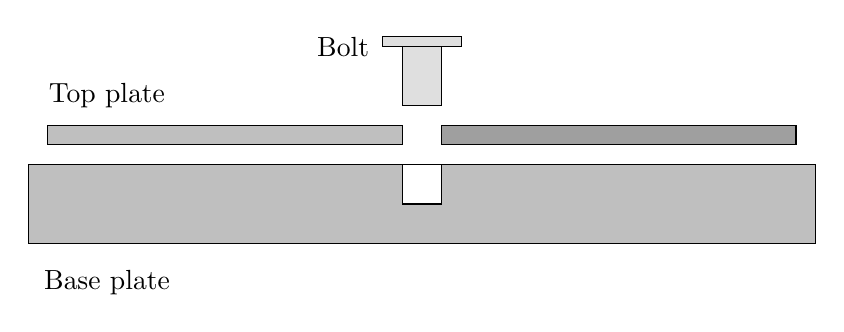
\begin{tikzpicture}
					\draw [fill=gray!50!white] (0,0) rectangle (10,1);
					\draw [draw=black,fill=white] (4.75,1) rectangle (5.25,0.5);
					\draw [fill=gray!50!white] (0.25,1.25) rectangle (4.75,1.5);
					\draw [fill=gray!75!white] (5.25,1.25) rectangle (9.75,1.5);
					\draw [fill=gray!25!white] (4.75,1.75) rectangle (5.25,2.5);
					\draw [fill=gray!25!white] (4.5,2.5) rectangle (5.5,2.625);
					\node at (4,2.5) {Bolt};
					\node at (1,1.875) {Top plate};
					\node at (1,-0.5) {Base plate};
				\end{tikzpicture}
			\caption{Three component system}
			\label{three_component}
			\end{center}
		\end{figure}
		The top plate is not free to move relative to the base plate. Since there is variation in the diameters of the holes and bolt and in the true positions of the holes due to manufacturing and/or assembly tolerances, there will be some chance that the alignment will be off enough that the bolt will not fit through the two holes. Monte Carlo analysis can be used in this situation to determine the probability of an arbitrary set of components fitting together and evaluating the tolerance specifications on the individual components and the alignment process.
		\begin{itemize}
			\item
			If the radius of the hole in the top plate is $r_p$, the radius of the hole in the base plate is $r_b$, the bolt diameter if $d$, and the relative misalignment of the two holes is $r$, determine the geometric criterion that can be used to determine whether the bolt will or will not fit into the assembly. Consider the following two cases: $r \geq \abs{r_p-r_b}$ and $r \leq \abs{r_p-r_b}$, as the ``fitting" criterion is different for the two cases. Refer to Figure~\ref{fit_criterion} for more details.
			\begin{figure}[!htbp]
				\begin{center}
				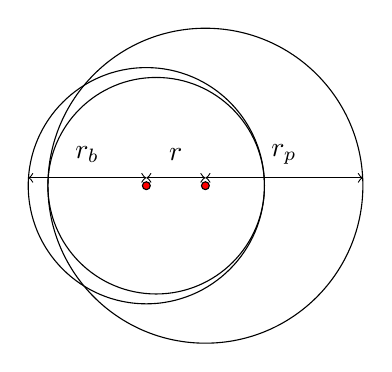
\begin{tikzpicture}
					\draw (0,0) circle (2);
					\draw (-0.75,0) circle (1.5);
					\draw (-0.625,0) circle (1.375);
					\draw [fill=red] (0,0) circle (0.05);
					\draw [fill=red] (-0.75,0) circle (0.05);
					\draw [<->] (0,0.1) -- (2,0.1);
					\draw [<->] (0,0.1) -- (-0.75,0.1);
					\draw [<->] (-0.75,0.1) -- (-2.25,0.1);
					\node at (1,0.4) {$r_p$};
					\node at (-0.375,0.4) {$r$};
					\node at (-1.5,0.4) {$r_b$};
				\end{tikzpicture}
				\caption{Fitting criterion}
				\label{fit_criterion}
				\end{center}
			\end{figure}
			\item
			Table~\ref{my_table} contains the nominal dimensions and $3\sigma$ tolerance limits for the radii of the two holes, the diameter of the bolt, and the $x$ and $y$ coordinates of the two holes measured with respect to some reference point. It is assumed that all the dimensions and coordinates are normally distributed.
			\begin{table}[!htbp]
				\caption{Dimensions for the problem}
				\label{my_table}
				\begin{center}
				\begin{tabular}{|c|c|c|}
					\hline
					\textbf{Item} & \textbf{Nominal value in mm} & \textbf{Tolerance $3\sigma$ in mm}\\
					\hline
					Bottom plate hole radius & $25.25$ & $\pm 0.05$\\
					\hline
					Top plate hole radius & $25.15$ & $\pm 0.05$\\
					\hline
					Bolt radius & $24.95$ & $\pm 0.21$\\
					\hline
					Top plate hole $x$-location & $100$ & $\pm 0.2$\\
					\hline
					Top plate hole $y$-location & $100$ & $\pm 0.2$\\
					\hline
					Bottom plate hole $x$-location & $100$ & $\pm 0.2$\\
					\hline
					Bottom plate hole $y$-location & $100$ & $\pm 0.2$\\
					\hline
				\end{tabular}
				\end{center}
			\end{table}
		\end{itemize}
		\item
		Consider a $4$ state Markov Chain whose probability transition matrix is given below:
		$$P = \begin{bmatrix}
		1-p & p & 0 & 0\\
		p & 1-2p & p & 0\\
		0 & p & 1-2p & p\\
		0 & 0 & p & 1-p
		\end{bmatrix}$$
		where $p=1/3$. Obtain the steady state distribution using simulation (count the fraction of times a state is visited by letting the Markov Chain evolve for $N=10^6$ time steps) and also by solving the appropriate set of equations.

		\item
		Evaluate the integral $$\int_0^1 \cos \bkt{2\pi \sqrt{1-x^2}}dx$$ by two different Monte Carlo techniques as indicated below. For both plot the convergence of the integrals as a function of $N$ (similar to the plot we obtained in class). Check whether the scaling of the intervals goes down as $1/\sqrt{N}$.
		\begin{itemize}
			\item
			\textbf{Method 1}: Generate $\{x_i\}_{i=1}^N$ that are uniformly distributed on the interval $[0,1]$ and compute the integral as the sample mean of the function values at these points.
			\item
			\textbf{Method 2}: Note that the function ranges from $0$ to $1$. Dump points $\{x_i,y_i\}_{i=1}^N$ on the unit square $[0,1]^2$ that are uniformly distributed and compute the integral by evaluating the fraction of points that lie below the function value.
		\end{itemize}
	\end{enumerate}
\end{document}